\documentclass{beamer}
\usetheme{Madrid}
\usecolortheme{beaver}
\usepackage{booktabs}
\usepackage{tikz}
\usetikzlibrary{positioning, arrows.meta}


% --- Title Information ---
\title[ACGN Multivariate Analysis]{Impact of Anime Creation Sources on Anime Quality}
\subtitle{A Multivariate Analysis with Bangumi Data}
\author{Hanwen Zhang, Jiahui Gu, Yihong Xiao} 
\date{December 17, 2025}

\begin{document}

% --- Slide 1: Title ---
\begin{frame}
    \titlepage
\end{frame}

% --- Slide 2: Introduction & Data ---
\begin{frame}{Introduction \& Data Source}
    \textbf{Thesis} \\
  This project will analyze the Impact of different anime creation sources on anime quality, with the relation-mapping of different genere adaptation.

    \vspace{0.5cm}

    \textbf{Data Source: Bangumi Archive}
    \begin{itemize}
        \item \textbf{Core Datasets:} \texttt{Subject.jsonlines} (Metadata with 580000 rows and 6 snapshots) and \texttt{Subject-relations.jsonlines} (Adaptation relations with 800000 rows).
        \item \textbf{Scale:} Modern dataset (1980--2025) containing thousands of entries.
        \item \textbf{Key Features Extracted:}
        \begin{itemize}
            \item \texttt{score} (User rating) \& \texttt{id} (generated by Bangumi server).
            \item \texttt{played\_amount, dropped\_amount } (Popularity).
            \item \texttt{type} (Novel, Manga, Anime, Game).
            \item \texttt{relation\_type}: adaptation.
        \end{itemize}
    \end{itemize}
\end{frame}

\begin{frame}{Data Processing Pipeline}
    \centering
    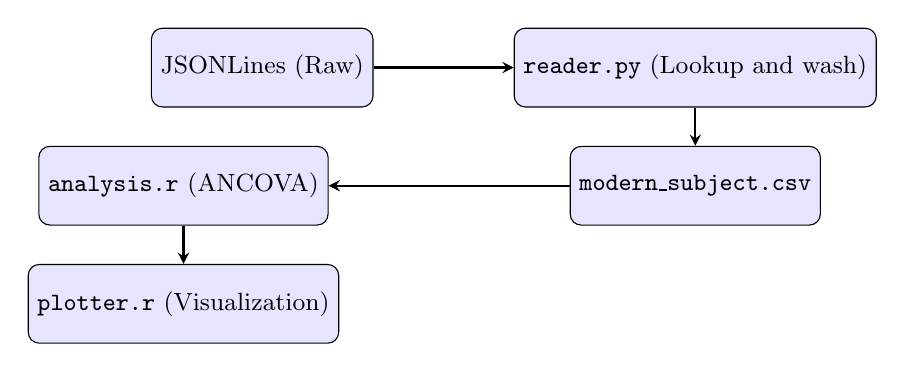
\begin{tikzpicture}[node distance=1.5cm]
        \tikzstyle{box} = [rectangle, rounded corners, minimum width=2.5cm, minimum height=1cm,text centered, draw=black, fill=blue!10]
        \tikzstyle{arrow} = [thick,->,>=stealth]
        
        \node (raw) [box] {\small JSONLines (Raw)};
        \node (reader) [box, right of=raw, xshift=4cm] {\small \texttt{reader.py} (Lookup and wash)};
        \node (modern) [box, below of=reader] {\small \texttt{modern\_subject.csv}};
        \node (analysis) [box, left of=modern, xshift=-5cm] {\small \texttt{analysis.r} (ANCOVA)};
        \node (plotter) [box, below of=analysis] {\small \texttt{plotter.r} (Visualization)};

        \draw [arrow] (raw) -- (reader);
        \draw [arrow] (reader) -- (modern);
        \draw [arrow] (modern) -- (analysis);
        \draw [arrow] (analysis) -- (plotter);
    \end{tikzpicture}
    
    \vspace{0.5cm}
    \begin{itemize}
    \item 
    \end{itemize}
\end{frame}






% --- Slide 3: Methodology ---
\begin{frame}{Methodology: The Adaptation Flow}
\scriptsize{
    \textbf{1. Relation Mapping} \\
   Paths to anime (e.g., Novel $\to$ Manga $\to$ Anime).

    \vspace{0.3cm}
    \begin{center}

\tikzstyle{every node}=[scale=0.3]
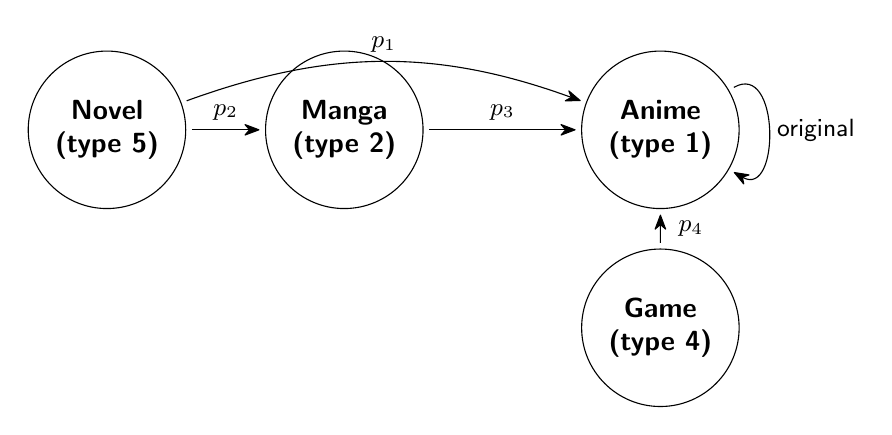
\begin{tikzpicture}[
    % Define standard styles for nodes and edges to keep code clean
    %set size
    scale=0.3,
    subject/.style={
        circle,
        draw=black,
        minimum size=2.0cm,
        font=\bfseries\sffamily,
        align=center,
        fill=white
    },
    relation/.style={
        -{Stealth[round, scale=1.3]}, % Nice arrowhead
        thin,
        shorten >=2pt, % Slight gap before touching the node
        shorten <=2pt  % Slight gap after leaving the node
    },
    label text/.style={
        midway,
        above,
        font=\sffamily\small
    }
]

    % --- 1. Place Nodes ---
    \node[subject] (novel) {Novel\\(type 5)};
    % Place manga 4cm to the right of novel
    \node[subject] (manga) [right=1cm of novel] {Manga\\(type 2)};
    % Place anime 4cm to the right of manga
    \node[subject] (anime) [right=2cm of manga] {Anime\\(type 1)};
    \node[subject] (game) [below =0.5cm of anime] {Game\\(type 4)};


    % --- 2. Draw Edges ---

    % Game -> Anime
    \draw[relation] (game) -- node[right, font=\sffamily\small, align=left] {\,\,$p_4$} (anime);

    % Novel -> Manga
    \draw[relation] (novel) -- node[label text] {$p_2$} (manga);

    % Manga -> Anime
    \draw[relation] (manga) -- node[label text] {$p_3$} (anime);

    % Novel -> Anime (Direct)
    % Using 'bend left' to curve it above the manga node
    \draw[relation] (novel) to[bend left=20] node[label text] {\small $p_1$} (anime);

    % Anime -> Anime (Self-pointing original)
    % Using a loop. Placed on the right side to avoid crowding the top arrows.
    \draw[relation] (anime) to [loop right, out=30, in=-30, min distance=2.5cm]
        node[right, font=\sffamily\small, align=left] {original} (anime);

    \end{tikzpicture}
    \end{center}

    \textbf{2. Statistical Model} \\
    Filter the mean anime score ($s_{anime}$) adjusted by one-year time interval.
    
    Setting: If $s_{anime} \geq s_{source}$, the adaptation is "successful or qualified".
    }
\end{frame}

% --- Slide 4: Preliminary Processing Results ---

\begin{frame}{Result: Descriptive Statistics}
    \begin{table}
        \centering
        \caption{Mean Scores by Source (Stable Anime)}
        \begin{tabular}{lrr}
            \toprule
            \textbf{Source Category} & \textbf{Mean Score} & \textbf{N (Count)} \\
            \midrule
            \textbf{Novel} & \textbf{6.59} & 1,880 \\
            Manga & 6.49 & \textbf{11,401} \\
            Original & 6.36 & 8,310 \\
            Game & 6.15 & 4,885 \\
            \bottomrule
        \end{tabular}
    \end{table}
    \vspace{0.3cm}
    \textit{Initial Finding: Manga or Novel have the highest raw mean, while Game adaptations has the lowest average quality.}
\end{frame}

\begin{frame}{Result Plot: Popularity vs Quality}
    \centering
    \includegraphics[width=0.55\textwidth]{plot_popularity_vs_quality.png}
    \begin{itemize}
        \item Positive correlation across all sources.
        \item \textbf{Selection Bias:} High-popularity titles tend to be better-funded adaptations.
    \end{itemize}
\end{frame}

\begin{frame}{Result Plot: Quality by Source}
    \centering
    \includegraphics[width=0.85\textwidth]{plot_quality_by_source.png}
    \begin{itemize}
        \item Novels show a higher "upper bond" for quality.
        \item Original anime show the widest variance (highest "risk").
    \end{itemize}
\end{frame}

\begin{frame}{Result Plot: Temporal Stability Using Linear Mixed Model}
    \centering
    \scriptsize
    \includegraphics[width=0.4\textwidth]{linear_mixed_model_result.png}
    \begin{itemize}
        \item \textbf{Monitoring:} Since all intercepts of interactions have calculated p-values {\scriptsize ($P_{calc} = 2Pr(Z > |t|)$)} close to zero at $0.01$ level, there is no significant interaction between \textit{Source} and \textit{Snapshot Date}.

$
     \text{Score}_{ij} = \beta_0 + \beta_1 \text{Source}_i + \beta_2 \text{ log(played\_amount)}_{ij} + \gamma_j(\text{Snapshot}_j) + (\text{Source}_i \times \text{Snapshot}_j) + u_j + \epsilon_{ij}
$


        \item Quality perceptions are stable over the 6-month data's time-snapshot interval(crossed two seasons).
    \end{itemize}
\end{frame}

% --- Slide 5: Citation & Conclusion ---
\begin{frame}{Citation \& Discussion}
    \begin{block}{Project Repository}
       \scriptsize ACGN-Biased-Multivariate-Analysis \\
        \scriptsize \url{https://github.com/CarlXerophilem/ACGN-Biased-Multivariate-Analysis}
    \end{block}

    \vspace{0.5cm}
    \begin{block}{Data Sources}
    \scriptsize \url{https://github.com/bangumi/Archive/releases/tag/archive}
    \end{block}
    \vspace{0.5cm}
    
    \textbf{Future Works:}
    \begin{itemize}
\scriptsize
        \item Complete tracking of adaptation paths across multiple ancestors.
        \item Segmentation of different animation subgenres (TV / Movie / OVA).

        \item Introduction of time-entropy related models to observe market trends (include js script for auto updating)...

    \end{itemize}
\end{frame}

\end{document}

